\bb
\ii Let $B=\{\boldv_1,\boldv_2,\dots ,\boldv_n\}$. Compute $\underset{B\rightarrow B'}{P}$ for each of the following bases $B'$, and explain what happens to coordinate vectors as we change from $B$ to $B'$. 
\\
(a) $B'=\{\boldv_2,\boldv_1,\boldv_3,\dots, \boldv_n\}$. 
\\
(b) $B'=\{3\boldv_1, 3\boldv_2,\dots , 3\boldv_n\}$. 
\\
\begin{solution}
\noindent In each case we will describe the change of basis matrix column by column, making use $\bolde_j$, the elements of the standard basis (or equivalently, the columns of the identity matrix). 

The computation of each column is done by inspection, since the new basis is closely related to the old one. 
\\
(a) We have $\underset{B\rightarrow B'}{P}=\begin{bmatrix}
\vert &\vert& &\vert\\
\bolde_2&\bolde_1&\cdots &\bolde_n\\
\vert &\vert& &\vert
\end{bmatrix}$.

When changing from $B$ to $B'$, simply swap the first two entries of the coordinate vector. 
\\
(b) We have $\underset{B\rightarrow B'}{P}=\begin{bmatrix}
\vert &\vert& &\vert\\
\frac{1}{3}\bolde_1&\frac{1}{3}\bolde_2&\cdots &\frac{1}{3}\bolde_n\\
\vert &\vert& &\vert
\end{bmatrix}$.

When changing from $B$ to $B'$, scale each entry of the coordinate vector by $1/3$. 
\end{solution}
\ii Let $V=P_1$ with basis $B'=\{2x+1, 3x+2\}$. 
\bb
\ii Compute $[p(x)]_{B'}$, where $p(x)=ax+b$, $a,b\in\R$. Your answer will be in terms of $a$ and $b$.
\ii Now do the same computation using a change of basis matrix involving the standard basis $B$.
\ee
\begin{solution}
\noindent (a) We seek the $c_1, c_2$ such that $c_1(2x+1)+c_2(3x+2)=ax+b$. This boils down to solving the matrix equation 
\[
\begin{bmatrix}
2&3\\
1&2
\end{bmatrix}
\begin{bmatrix}
c_1\\ c_2
\end{bmatrix}
=\begin{bmatrix}
a\\ b
\end{bmatrix}
\Longleftrightarrow \begin{bmatrix}
c_1\\ c_2
\end{bmatrix}=\left(\begin{bmatrix}
2&3\\
1&2
\end{bmatrix}\right)^{-1}\begin{bmatrix}
a\\ b
\end{bmatrix}=\begin{bmatrix}
2a-3b\\ -a+2b
\end{bmatrix}
\]
(b) To do the same computation with a change of basis matrix, we let $B=\{x, 1\}$. Then $\underset{B'\rightarrow B}{P}=\begin{bmatrix}
2&3\\
1&2
\end{bmatrix}$, and hence 
\[
\underset{B\rightarrow B'}{P}=\left(\begin{bmatrix}
2&3\\
1&2
\end{bmatrix}\right)^{-1}=\begin{bmatrix}
2&-3\\
-1&2
\end{bmatrix}
.
\]
Thus 
\[
[ax+b]_{B'}= \underset{B\rightarrow B'}{P}[ax+b]_B=\begin{bmatrix}
2&-3\\
-1&2
\end{bmatrix}
\begin{bmatrix}
a\\ b
\end{bmatrix}=
\begin{bmatrix}
2a-3b\\
-a+2b
\end{bmatrix}
.
\]

\end{solution}
\ii Let $V$ be a finite-dimensional vector space, and let $B$, $B'$, $B''$ be three different bases of $V$. Let $P=\underset{B\rightarrow B'}{P}$ and $Q=\underset{B\rightarrow B''}{P}$. 
\bb
\ii Express $\underset{B'\rightarrow B''}{P}$ in terms of $P$, $Q$, and/or their inverses. 

Verify that your matrix satisfies the defining property of the change of basis matrix. 
\ii Utilize the formula in (a) to compute $\underset{B'\rightarrow B''}{P}$, where $B'=\{2x+1, 3x+2\}$ and $B''=\{x-1,x+1\}$: two nonstandard bases of $P_1$. 
\ee
\begin{solution}
\noindent (a) I claim $\underset{B'\rightarrow B''}{P}=QP^{-1}$ To verify the claim, I need only show that $QP^{-1}$ satisfies the defining property: i.e., $QP^{-1}[\boldv]_{B'}=[\boldv]_{B''}$ for all $\boldv\in V$. We compute
\begin{align*}
QP^{-1}[\boldv]_{B'}&=Q\underset{B'\rightarrow B}{P}[\boldv]_{B'} &\left(\underset{B'\rightarrow B}{P}=(\underset{B\rightarrow B'}{P})^{-1}\right)\\
&=Q[\boldv]_{B}\\
&=[\boldv]_{B''} &(Q=\underset{B\rightarrow B''}{P})
\end{align*}
This proves that $QP^{-1}=\underset{B'\rightarrow B''}{P}$. 
\vspace{.1in}
\\
(b) Let $B=\{x, 1\}$. Then we have $\underset{B'\rightarrow B}{P}=\begin{bmatrix}
2&3\\
1&2
\end{bmatrix}$, and $\underset{B\rightarrow B''}{P}=\begin{bmatrix}
1&1\\
-1&1
\end{bmatrix}^{-1}=\frac{1}{2}\begin{bmatrix}
1&-1\\
1&1
\end{bmatrix}$. 
\\
We have 
\[
\underset{B'\rightarrow B''}{P}=\underset{B\rightarrow B''}{P}\underset{B'\rightarrow B}{P}=\frac{1}{2}\begin{bmatrix}
1&-1\\
1&1
\end{bmatrix}
\begin{bmatrix}
2&3\\
1&2
\end{bmatrix}
=\frac{1}{2}\begin{bmatrix}
1&1\\
3&5
\end{bmatrix}
\]
\end{solution}
\ii Let $B$, $B'$, and $B''$ be three different bases for a finite dimensional vector space $V$. Show that 
\[
\underset{B\rightarrow B''}{P}=\underset{B'\rightarrow B''}{P}\cdot \underset{B\rightarrow B'}{P} 
\]
using only the defining property and uniqueness of change of basis matrices. 
\\
\begin{solution}
%\ \\
\noindent Let $C=\underset{B'\rightarrow B''}{P}\cdot \underset{B\rightarrow B'}{P} 
$. Then we have 
\begin{align*}
C[\boldv]_B&=\underset{B'\rightarrow B''}{P}\cdot \underset{B\rightarrow B'}{P} 
[\boldv]_B\\
&=\underset{B'\rightarrow B''}{P}(\underset{B\rightarrow B'}{P} 
[\boldv]_B)\\
&=\underset{B'\rightarrow B''}{P}[\boldv]_{B'} &\text{(prop. of $\underset{B\rightarrow B'}{P}$) }\\
&=[\boldv]_{B''} &\text{(prop. of $\underset{B'\rightarrow B''}{P}$) }.
\end{align*}
Thus $C[\boldv]_B=[\boldv]_{B''}$ for all $\boldv\in V$, which is the defining property of $\underset{B\rightarrow B''}{P}$. By {\em uniqueness} it follows that $C=\underset{B\rightarrow B''}{P}$.
\end{solution}
\ii True or false. If true, provide a proof; if false, give an explicit counterexample. 
\bb
\ii If $B$ is a basis for an $n$-dimensional space $V$, then $\underset{B\rightarrow B}{P}=I_n$. 
\ii If $\underset{B\rightarrow B'}{P}$ is diagonal, then each basis element of $B$ is a scalar multiple of some basis element of $B'$. 
\ii If each basis element of $B'$ is a scalar multiple of {\em some} basis element of $B$, then $\underset{B\rightarrow B'}{P}$ is diagonal. 
\ii The coordinate vector of a vector $\boldx$ in $\R^n$ relative to the standard basis for $\R^n$ is $\boldx$.
\ee
\begin{solution}
\noindent
(a) True. We show this in the lecture notes. 
\\
(b) True. Since $\underset{B\rightarrow B'}{P}$ is diagonal, so is its inverse $\underset{B\rightarrow B'}{P}^{-1}=\underset{B'\rightarrow B}{P}$. The $j$-th column of this matrix is, using the change of basis formula, just $[\boldv_j']_B$, where $\boldv_j'$ is the $j$-th element of $B'$. Since the matrix is diagonal, this column vector is of the form $c_j\bolde_j$ for some $c_j\in\R$. Unpacking the definition of the coordinate vector, this means simply that $\boldv_j=c_j\bolde_j$ for some $c_j\in \R$. So in fact the $j$-th element of $B'$ is a scalar multiple {\color{red}of the $j$-th element of $B$} (not just any element). 
\\
(c) False. As the color in the previous solution emphasizes, to be diagonal we need the $j$-th element of $B'$ to be a scalar multiple of the $j$-th element of $B$. Consider the bases $B=\{(1,0), (0,1)\}$ and $B'=\{(0,1), (1,0)\}$ of $\R^2$. Then the elements of $B'$ are scalar multiples of elements of $B$, but $\underset{B\rightarrow B'}{P}=\begin{bmatrix}
0&1\\
1&0
\end{bmatrix}$ is not diagonal.  
\\
(d) True. Let $B$ be the standard basis, and let $\bolde_i$ be the $i$-th element $B$: i.e., $\bolde_i$ has a 1 in the $i$-th entry, and 0's elsewhere. Given any $\boldv=(a_1,a_2,\dots, a_n)$, we have $\boldv=a_1\bolde_1+a_2\bolde_2+\cdots +a_n\bolde_n$, as we have remarked before. By definition, we then have $[\boldv]_B=(a_1,a_2,\dots, a_n)=\boldv$. 
\end{solution}
\ii Consider the bases $B = \{p_1 = 6 +3x, p_2 = 10+2x\}$ and $B'=\{q_1=2, q_2=3+2x\}$ for $P_1$.
\bb
\ii Compute the transition matrix from $B'$ to $B$.
\ii Compute the transition matrix from $B$ to $B'$.
\ii Compute the coordinate vector $[p]_B$, where $p = -4 +x$ and use the change of basis formula theorem to compute $[p]_{B'}$.
\ii Now compute $[p]_{B'}$ directly and verify that your answer agrees with part (c). 
\ee
\begin{solution}
\noindent To compute the transition matrix from $B'$ to $B$ place the bases in a matrix, with the new basis on the left and the old basis on the right, and use row operations to reduce the left side to the identity.
$$
\begin{bmatrix}[cc|cc]
6&10&2&3\\
3&2&0&2
\end{bmatrix}
\rightarrow
\begin{bmatrix}[cc|cc]
1&0&-2/9&7/9\\
0&1&1/3&-1/6
\end{bmatrix}
$$
Thus transition matrix from $B'$ to $B$ is
$$
\begin{bmatrix}[cc]
-2/9&7/9\\
1/3&-1/6
\end{bmatrix}
$$
Similarly, we can find the transition matrix from $B$ to $B'$
$$
\begin{bmatrix}[cc|cc]
2&3&6&10\\
0&2&3&2
\end{bmatrix}
\rightarrow
\begin{bmatrix}[cc|cc]
1&0&3/4&7/2\\
0&1&3/2&1
\end{bmatrix}
$$
Thus transition matrix from $B$ to $B'$ is
$$
\begin{bmatrix}[cc]
3/4&7/2\\
3/2&1
\end{bmatrix}
$$
Computing $[p]_B$ directly we can see
$$
\begin{bmatrix}[cc|c]
6&10&-4\\
3&2&1
\end{bmatrix}
\rightarrow
\begin{bmatrix}[cc|c]
1&0&1\\
0&1&-1
\end{bmatrix}
$$
Thus
$$
[p]_B =
\begin{bmatrix}[c]
1\\
-1
\end{bmatrix}
$$
Using formula $(12)$, we can find $[p]_{B'}$
$$
[p]_{B'} =
\begin{bmatrix}[cc]
3/4&7/2\\
3/2&1
\end{bmatrix}
\begin{bmatrix}[c]
1\\
-1
\end{bmatrix}=
\begin{bmatrix}[c]
-11/4\\
1/2
\end{bmatrix}
$$
Finally if we compute $[p]_{B'}$ directly we will arrive at the same answer.
$$
\begin{bmatrix}[cc|c]
2&3&-4\\
0&2&1
\end{bmatrix}
\rightarrow
\begin{bmatrix}[cc|c]
1&0&-11/4\\
0&1&1/2
\end{bmatrix}
$$
Thus
$$
[p]_{B'} =
\begin{bmatrix}[c]
-11/4\\
1/2
\end{bmatrix}
$$
\end{solution}

\ii Let $B$ be the standard basis for $\R^3$, and let $B' = \{\boldv_1,\boldv_2,\boldv_3\}$ where $\boldv_1 = (1,2,1)$, $\boldv_2 = (2,5,0)$, and $\boldv_3 = (3,3,8)$. 
\bb
\ii Compute $\underset{B'\rightarrow B}{P}$. 
\ii Now compute $\underset{B\rightarrow B'}{P}$.
\ii Confirm these two matrices are inverses of one another.
\ii Let $\boldw = (5,-3,1)$. Compute $[\boldw]_{B'}$ directly, then compute $[\boldw]_{B'}$ using $[\boldw]_{B}$ and the relevant change of basis matrix. 
\ii Let $\boldw = (3,-5,0)$. Compute $[\boldw]_{B}$ by inspection, then compute $[\boldw]_{B'}$ using $[\boldw]_{B}$ and the relevant transition matrix.
\ee
\begin{solution}
\noindent 
(a) By inspection
$$
\underset{B'\rightarrow B}{P} =
\begin{bmatrix}[ccc]
1&2&3\\
2&5&3\\
1&0&8
\end{bmatrix}
$$
(b) We now compute $\underset{B\rightarrow B'}{P}=(\underset{B'\rightarrow B}{P})^{-1}$. Using formula (14)
$$
\begin{bmatrix}[ccc|ccc]
1&2&3&1&0&0\\
2&5&3&0&1&0\\
1&0&8&0&0&1
\end{bmatrix}
\rightarrow
\begin{bmatrix}[ccc|ccc]
1&0&0&-40&16&9\\
0&1&0&13&-5&-3\\
0&0&1&5&-2&-1
\end{bmatrix}
$$
we can see that
$$
\underset{B\rightarrow B'}{P}=
\begin{bmatrix}[ccc]
-40&16&9\\
13&-5&-3\\
5&-2&-1
\end{bmatrix}
$$
(c) It is easy to see that these are inverses
$$
\begin{bmatrix}[ccc]
1&2&3\\
2&5&3\\
1&0&8
\end{bmatrix}
\begin{bmatrix}[ccc]
-40&16&9\\
13&-5&-3\\
5&-2&-1
\end{bmatrix}
=
\begin{bmatrix}[ccc]
1&0&0\\
0&1&0\\
0&0&1
\end{bmatrix}
$$
(d) Calculating $[\boldw]_{B'}$ directly
$$
\begin{bmatrix}[ccc|c]
1&2&3&5\\
2&5&3&-3\\
1&0&8&1
\end{bmatrix}
\rightarrow
\begin{bmatrix}[ccc|c]
1&0&0&-239\\
0&1&0&77\\
0&0&1&30
\end{bmatrix}
$$
Thus 
$$
[\boldw]_{B'} =
\begin{bmatrix}[c]
-239\\
77\\
30
\end{bmatrix}
$$
Now using change of basis
$$
[\boldw]_{B'} =\underset{B\rightarrow B'}{P}[\boldw]_B=
\begin{bmatrix}[ccc]
-40&16&9\\
13&-5&-3\\
5&-2&-1
\end{bmatrix}
\begin{bmatrix}[c]
5\\
-3\\
1
\end{bmatrix}=
\begin{bmatrix}[c]
-239\\
77\\
30
\end{bmatrix}
$$
(e) By inspection we have $[(-3,5,0)]_B=(-3,5,0)$. Then, using our change of basis matrix, we have 
$$
[\boldw]_{B'} =
\begin{bmatrix}[ccc]
-40&16&9\\
13&-5&-3\\
5&-2&-1
\end{bmatrix}
\begin{bmatrix}[c]
3\\
-5\\
0
\end{bmatrix}=
\begin{bmatrix}[c]
-200\\
64\\
25
\end{bmatrix}
$$
\end{solution}
\ii The matrix
$$
\begin{bmatrix}[ccc]
1&0&0\\
0&3&2\\
0&1&1
\end{bmatrix}
$$
is the change of basis matrix from what basis $B$ to the basis $\{(1,1,1),(1,1,0),(1,0,0)\}$ in $\R^3$?
\\
\begin{solution}
Let $B = \{(a,b,c),(d,e,f),(h,g,i)\}$
Then
\begin{eqnarray*}
(a,b,c) &=& 1(1,1,1) + 0(1,1,0) + 0(1,0,0) = (1,1,1)\\
(d,e,f) &=& 0(1,1,1) + 3(1,1,0) + 1(1,0,0) = (4,3,0)\\
(g,h,i) &=& 0(1,1,1) + 2(1,1,0) + 1(1,0,0) = (3,2,0)
\end{eqnarray*}
Thus $B = \{(1,1,1),(4,3,0),(3,2,0)\}$. We can even double check this by using formula (14)
$$
\begin{bmatrix}[ccc|ccc]
1&1&1&1&4&3\\
1&1&0&1&3&2\\
1&0&0&1&0&0
\end{bmatrix}
\rightarrow
\begin{bmatrix}[ccc|ccc]
1&0&0&1&0&0\\
0&1&0&0&3&2\\
0&0&1&0&1&1
\end{bmatrix}
$$
\end{solution}

%\ii Let $T_{\alpha}\colon\R^2\rightarrow\R^2$ be reflection through the line $\ell_{\alpha}$, as defined previously in  Recall also that $T_{\alpha}$ is an origin-fixing isometry, hence a linear transformation. 
%\\
%Compute the matrix $A$ such that $T_{\alpha}=T_A$ as follows: first compute $A'=[T_{\alpha}]_{B'}$ where $B'=\{\boldv_1,\boldv_2\}$ is a basis for $\R^2$ satisfying $\boldv_1\in \ell_\alpha$, $\boldv_2\in \ell_\alpha^\perp$; then compute $A=[T_{\alpha}]_B$ from $A'$ using the change of basis formula for transformations. 
%\\
%Note: your vectors $\boldv_1, \boldv_2$ will be expressed in terms of $\alpha$ (and some trig functions). 
%\\
%Check that you get the same answer from before! 
%\\
%\begin{solution} 
%%\ \\
%\noindent 
%Since $B$ is the standard basis, it turns out that The matrix $A=[T]_B$ is just the matrix that defines the given linear transformation. We computed this in an earlier exercise. We got
%\[
%A=\begin{bmatrix}[rr]
%\cos(2\alpha)&\sin(2\alpha)\\
%\sin(2\alpha)&-\cos(2\alpha)
%\end{bmatrix}=\begin{bmatrix}[rr]
%-1/2&\sqrt{3}/2\\
%\sqrt{3}/2&1/2
%\end{bmatrix}.
%\]
%Given a basis as specified, the matrix $A'=[T]_{B'}$ is simpler because the action of $T$ on this basis is simpler: $T(\boldv_1)=\boldv_1$ and $T(\boldv_2)=-\boldv_2$ (draw a picture!). Thus 
%\[
%A'=\begin{bmatrix}
%\vert&\vert\\
%[T(\boldv_1)]_{B'}&[T(\boldv_2)]_{B'}\\
%\vert&\vert
%\end{bmatrix}
%=\begin{bmatrix}
%\vert&\vert\\
%[\boldv_1]_{B'}&[-\boldv_2]_{B'}\\
%\vert&\vert
%\end{bmatrix}=
%\begin{bmatrix}[rr]
%1&0\\
%0&-1
%\end{bmatrix}.
%\]
%Let's actually pin down a basis $B'$ as specified. The basis elements are necessarily orthogonal (from the description); I will make them orthonormal to make my life as easy as possible!  The vector $\boldv_1$ points along $\ell_{\alpha}$: a unit vector fitting this description is $\boldv_1=(\cos(\alpha), \sin(\alpha))$. The vector $\boldv_2$ should be a unit vector orthogonal to $\boldv_1$: I pick $\boldv_2=(-\sin(\alpha), \cos(\alpha))$. 
%
%We need to compute change of bases matrices between $B'$ and the standard basis $B$. Again we find ourselves in the special setting where $\underset{B'\rightarrow B}{P}$ is built by simply putting the elements of $B'$ as its columns. Thus we have 
%\begin{align*}
%\underset{B'\rightarrow B}{P}&=\begin{bmatrix}
%[rr]
%\cos(\alpha) &-\sin(\alpha)\\
%\sin(\alpha)&\cos(\alpha)
%\end{bmatrix}\\
%\\
%\underset{B\rightarrow B'}{P}&=(\underset{B'\rightarrow B}{P})^{-1}\\
%&=(\underset{B'\rightarrow B}{P})^{T} &\text{(since columns of $\underset{B'\rightarrow B}{P}$ are orthonormal!}\\
%&=\begin{bmatrix}
%[rr]
%\cos(\alpha) &\sin(\alpha)\\
%-\sin(\alpha)&\cos(\alpha)
%\end{bmatrix}
%\end{align*}
%Lastly, we compute 
%\begin{align*}
%A=[T]_B&=(\underset{B\rightarrow B'}{P})^{-1}[T]_{B'}\underset{B\rightarrow B'}{P}\\
%&=\underset{B'\rightarrow B}{P}[T]_{B'}\underset{B\rightarrow B'}{P}\\
%&=\begin{bmatrix}
%[rr]
%\cos(\alpha) &-\sin(\alpha)\\
%\sin(\alpha)&\cos(\alpha)
%\end{bmatrix}
%\begin{bmatrix}[rr]
%1&0\\
%0&-1
%\end{bmatrix}
%\begin{bmatrix}
%[rr]
%\cos(\alpha) &\sin(\alpha)\\
%-\sin(\alpha)&\cos(\alpha)
%\end{bmatrix}\\
%&=
%\begin{bmatrix}
%\cos^2(\alpha)-\sin^2(\alpha) & 2\sin(\alpha)\cos(\alpha)\\
%2\sin(\alpha)\cos(\alpha)&\sin^2(\alpha)-\cos^2(\alpha)
%\end{bmatrix}
%\\
%&=\begin{bmatrix}[rr]
%\cos(2\alpha)&\sin(2\alpha)\\
%\sin(2\alpha)&-\cos(2\alpha)
%\end{bmatrix}. \ \checkmark
%\end{align*}
%\end{solution}
\ii Define $T\colon \R^3\rightarrow\R^3$ as 
$$
T(x_1,x_2,x_3) = (x_1+2x_2-x_3,-x_2,x_1+7x_3)
$$
Let $B$ be the standard basis of $\R^3$, and let $B'$ be the nonstandard basis 
$$
B' = \{(1,0,0),(1,1,0),(1,1,1)\}.
$$
First compute $[T]_B$, then compute $[T]_{B'}$ using the change of basis formula for transformations. 
\\
\begin{solution}
%\ \\
\noindent
Start by using $T$ on each vector in the standard basis
\begin{eqnarray*}
T((1,0,0)) &=& (1,0,1)\\
T((0,1,0)) &=& (2,-1,0)\\
T((0,0,1)) &=& (-1,0,7)
\end{eqnarray*}
Then we can take these as the columns of $[T]_B$.
$$
[T]_B =
\begin{bmatrix}[ccc]
1&2&-1\\
0&-1&0\\
1&0&7
\end{bmatrix}
$$
According to the change of basis formula, we have  $[T]_{B'} = P_{B\rightarrow B'}[T]_BP_{B'\rightarrow B}$. 
Recall that in this very specific context ($V=\R^n$, $B$ the standard basis) the change of basis matrix $\underset{B'\rightarrow B}{P}$ is obtained by simply placing the elements of $B'$ as the columns of a vector: 
\[
P_{B'\rightarrow B} =
\begin{bmatrix}[ccc]
1&1&1\\
0&1&1\\
0&0&1
\end{bmatrix}
\]
Then we have 
\[
\underset{B\rightarrow B'}{P}=(\underset{B'\rightarrow B}{P})^{-1}=
\begin{bmatrix}[ccc]
1&-1&0\\
0&1&-1\\
0&0&1
\end{bmatrix}
\]

Now we can use the change of basis formula to compute 
\[
[T]_{B'} = 
\begin{bmatrix}[rrr]
1&-1&0\\
0&1&-1\\
0&0&1
\end{bmatrix}
\begin{bmatrix}[rrr]
1&2&-1\\
0&-1&0\\
1&0&7
\end{bmatrix}
\begin{bmatrix}[rrr]
1&1&1\\
0&1&1\\
0&0&1
\end{bmatrix} =
\begin{bmatrix}[rrr]
1&4&3\\
-1&-2&-9\\
1&1&8
\end{bmatrix}
\]
\end{solution}
\ii Define $T\colon P_1\rightarrow P_1$ as 
$$
T(a_0 +a_1x) = a_0 +a_1(x+1) = (a_0 +a_1) +a_1x.
$$
The following are two different bases for $P_1$: $B = \{6+3x, 10+2x\}$; $B' = \{2,3+2x\}$.
\\
First compute $[T]_B$, then use the change of basis formula for transformations to compute $[T]_{B'}$. 
\\
\begin{solution}
%\ \\
\noindent In a similar fashion to the last problem
\begin{eqnarray*}
 [T(6+3x)]_B &=& [9+3x]_B=(2/3, 1/2) \\
 \left[T(10+2x)\right]_B &=& [12 +2x]_B=(-2/9,4/3)
\end{eqnarray*}
Thus
$$
[T]_B =
\begin{bmatrix}[rr]
2/3&-2/9\\
1/2&4/3
\end{bmatrix}
$$
We compute $P_{B\rightarrow B'}$ using the recipe
$$
P_{B\rightarrow B'} =\begin{bmatrix}
\vert&\vert \\
[6+3x]_{B'}&[10+2x]_{B'}\\
\vert&\vert
\end{bmatrix}
=
\begin{bmatrix}[cc]
3/4&7/2\\
3/2&1
\end{bmatrix}
$$
Then 
$$P_{B'\rightarrow B}=(P_{B\rightarrow B'})^{-1}=
\begin{bmatrix}[cc]
-2/9&7/9\\
1/3&-1/6
\end{bmatrix}
$$
Then we have 
$$
[T]_{B'} =
\begin{bmatrix}[cc]
3/4&7/2\\
3/2&1
\end{bmatrix}
\begin{bmatrix}[rr]
2/3&-2/9\\
1/2&4/3
\end{bmatrix}
\begin{bmatrix}[cc]
-2/9&7/9\\
1/3&-1/6
\end{bmatrix}
=
\begin{bmatrix}[cc]
1&1\\
0&1
\end{bmatrix}
$$
\end{solution}
\ii Let $T\colon V\rightarrow W$ be a linear transformation between two finite-dimensional vector spaces. 

Suppose $B_1, B_2$ are two different bases of $V$, and $B_1', B_2'$ are two different bases of $W$. 

State and prove a matrix equation relating $[T]_{B_2}^{B_2'}$ in terms of $[T]_{B_1}^{B_1'}$, $\underset{B_1\rightarrow B_2}{P}$, $\underset{B_1'\rightarrow B_2'}{P}$,  and/or the inverses of these change of basis matrices. 

To prove your equality, you should show that the LHS and RHS matrices both satisfy the defining property of $[T]_{B_2}^{B_2'}$. 
\\
\begin{solution}
\noindent
I claim 
\[
[T]_{B_2}^{B_2'}=\underset{B_1'\rightarrow B_2'}{P}\ [T]_{B_1}^{B_1'}\ \underset{B_2\rightarrow B_1}{P}=\underset{B_1'\rightarrow B_2'}{P}\ [T]_{B_1}^{B_1'}\ (\underset{B_1\rightarrow B_2}{P})^{-1}
\]
To prove the claim, I need only show the matrix on the RHS, call it $C$, satisfies the defining property of $[T]_{B_2}^{B_2'}$: namely, 
\[
C[\boldv]_{B_2}=[T(\boldv)]_{B_2'} \text{ for all $\boldv\in V$}.
\]
To this end we compute:
\begin{align*}
\underset{B_1'\rightarrow B_2'}{P}\ [T]_{B_1}^{B_1'}\ \underset{B_2\rightarrow B_1}{P}[\boldv]_{B_2}&=\underset{B_1'\rightarrow B_2'}{P}\ [T]_{B_1}^{B_1'}[\boldv]_{B_1} &\text{(convert to $B_1$ coordinates)}\\
&=\underset{B_1'\rightarrow B_2'}{P}[T(\boldv)]_{B_1'} &\text{(defining property of $[T]_{B_1}^{B_1'}$)}\\
&=[T(\boldv)]_{B_2'} &\text{(convert to $B_2'$-coordinates)}
\end{align*}
\end{solution}
\ii Suppose $T\colon \mathbb{R}^2\rightarrow\mathbb{R}^2$ is a linear transformation, and that for any vector $\mathbf{v}$ of the form $\mathbf{v}=c(1,1)+d(-1,1)$, we have 
\[
T(\mathbf{v})=T\left(c(1,1)+d(-1,1)\right)=(c+d)(1,1)+d(-1,1).
\]
Note: this is an example of a {\em shearing transformation} along the vector $(1,1)$. 
\bb
\ii Let $B'=\{(1,1), (-1,1)\}$. Compute $[T]_{B'}$. 
\ii Use the change of basis formula to compute $A=[T]_B$, where $B$ is the standard basis. 
\ii Compute $T(1,2)$. 
\ee
\begin{solution}
\noindent
(a) We compute $T(1,1)=T\left(1(1,1)+0(-1,1)\right)=(1+0)(1,1)+0(-1,1)=(1,1)$. Thus $[T(1,1)]_{B'}=(1,0)$. 

Similarly, $T(-1,1)=T\left( 0(1,1)+1(-1,1)\right)=1(1,1)+1(-1,1)$. Thus $[T(-1,1)]_{B'}=(1,1)$. 

It follows that $[T]_{B'}=\begin{bmatrix}
1&1\\
0&1
\end{bmatrix}$.
\\
(b) As usual we see by inspection that $\underset{B'\rightarrow B}{P}=\begin{bmatrix}
1&-1\\
1&1
\end{bmatrix}$. 

Using inverses we then compute $\underset{B\rightarrow B'}{P}=\frac{1}{2}\begin{bmatrix}
1&1\\
-1&1
\end{bmatrix}$. 

Thus 
\[
[T]_B=\underset{B'\rightarrow B}{P}[T]_{B'}\underset{B\rightarrow B'}{P}=\frac{1}{2}\begin{bmatrix}
1&-1\\
1&1
\end{bmatrix}\begin{bmatrix}
1&1\\
0&1
\end{bmatrix}\begin{bmatrix}
1&1\\
-1&1
\end{bmatrix}=\frac{1}{2}\begin{bmatrix}
1&1\\
-1&3
\end{bmatrix}.
\]
(c) We have 
\[
T(1,2)=A\begin{bmatrix}
1\\2
\end{bmatrix}=\frac{1}{2}\begin{bmatrix}
1&1\\
-1&3
\end{bmatrix}
\begin{bmatrix}
1\\ 2
\end{bmatrix}
=
\frac{1}{2}\begin{bmatrix}
3\\
5
\end{bmatrix}
\]
\end{solution}

\ii For fixed direction vector $\boldd=(a,b)\ne \boldzero$, let $\ell$ be the line in $\R^2$ passing through the origin that it defines. 
\\
Define $T\colon \R^2\rightarrow\R^2$ to be reflection through $\ell$, as defined in Exercise \ref{ex:linereflection} of Section 3.2. Recall that $T$ is a linear transformation. 
\bb
\ii Construct a basis $B'$ of $\R^2$ which pays attention to the geometry involved in the definition of $T$, and compute $[T]_{B'}$. 

(If you picked your basis appropriately, $[T]_{B'}$ should be diagonal.) 
\ii Now use the change of basis formula to compute the $A$ such that $T=T_A$. 
\ee
\begin{solution}
\noindent
(a) I pick my basis to be $B'=\{\boldv_1, \boldv_2\}$, where $\boldv_1=(a,b)=\boldd$, the direction vector of $\ell$, and $\boldv_2=(-b,a)$, a vector pointing orthogonally to $\ell$. 

First observe that $T(\boldv_1)=\boldv_1$. This is because $\boldv_1$ lies on $\ell$, and the reflection of a point that lies on $\ell$ is equal to itself. 

Next, observe that $T(\boldv_2)=-\boldv_2$. This is because $\boldv_2$ points orthogonally to $\ell$, so its orthogonal projection onto $\ell$ is just $\boldzero$, and its reflection is thus $-\boldv_2$. (As usual, I conflate vectors with points in this discussion.) See picture below. 
\[
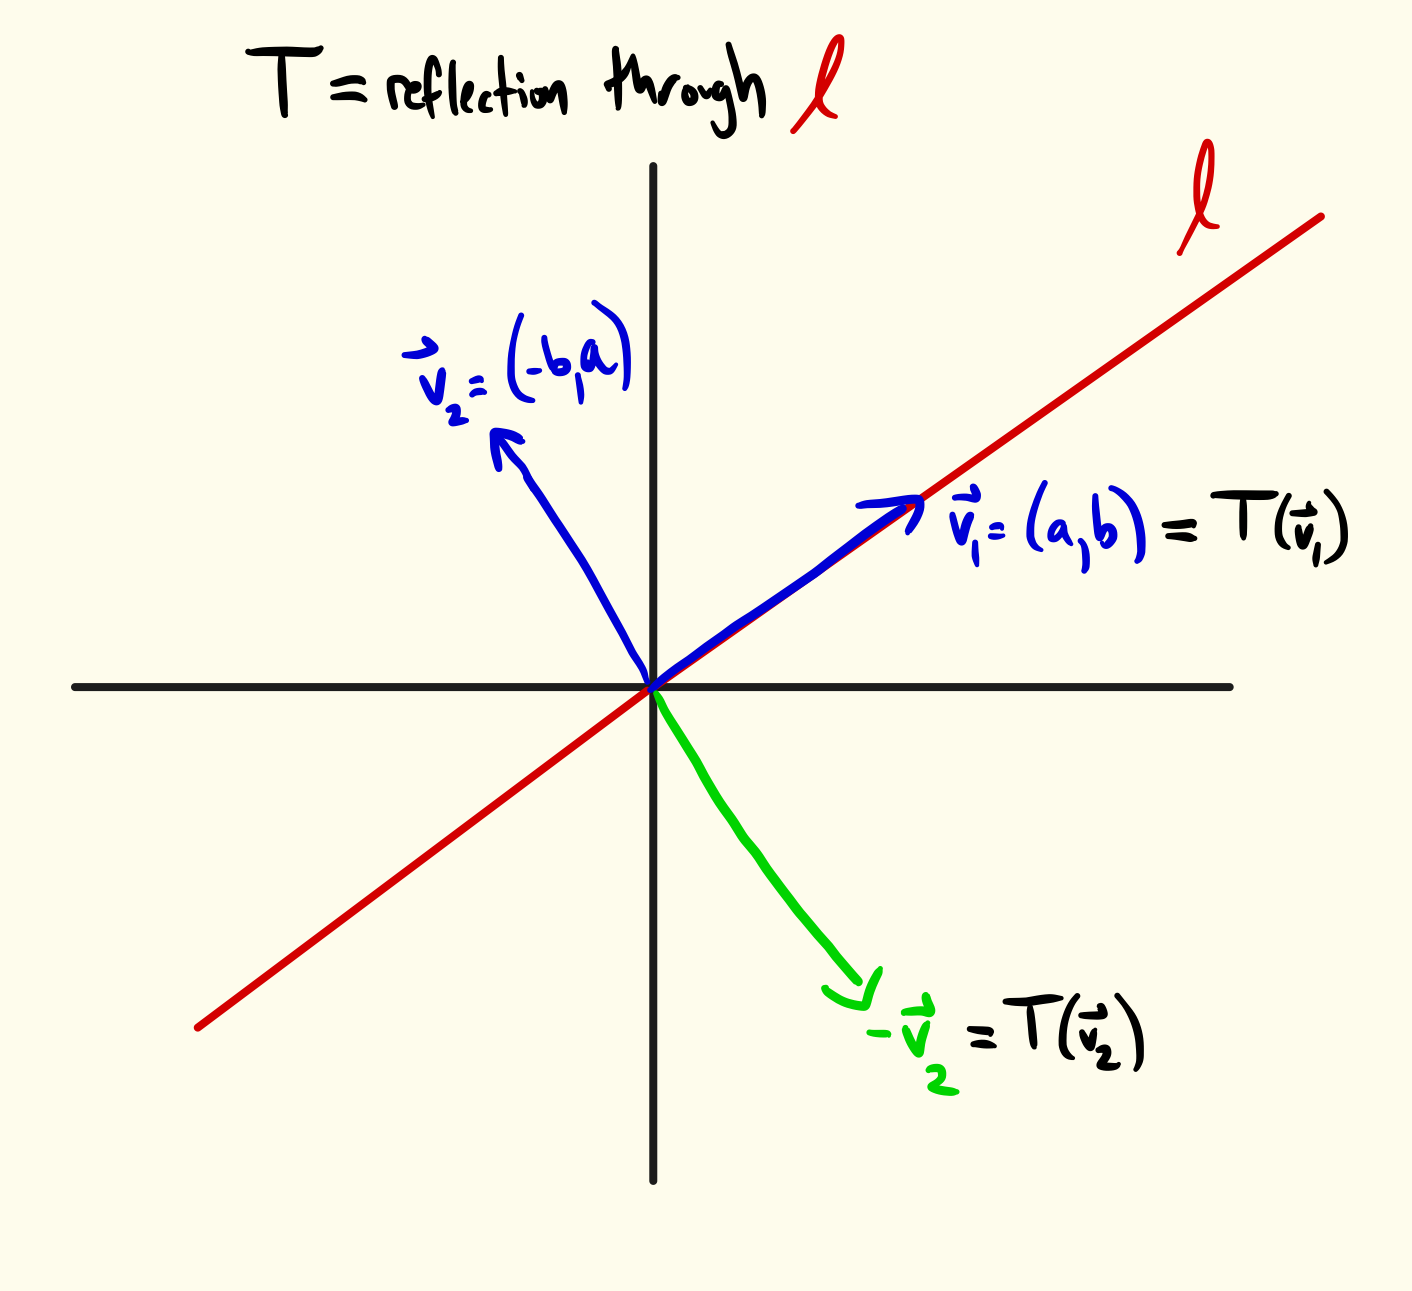
\includegraphics[width=4in]{../Lectures/Images/LineReflection}
\] 
Then we have 
\[
[T]_{B'}=\begin{bmatrix} \vert &\vert \\ [T(\boldv_1)]_{B'} & [T(\boldv_2)]_{B'}\\ \vert &\vert \end{bmatrix}=\begin{bmatrix} \vert &\vert \\ [\boldv_1]_{B'} & [-\boldv_2]_{B'}\\ \vert &\vert \end{bmatrix}=\begin{bmatrix}[rr]
1&0\\
0&-1
\end{bmatrix}.
\]
(b) To compute the $A$ such that $T=T_A$, note that $A=[T]_B$ where $B$ is the standard basis of $\R^2$. We can then use the change of basis formula: 
\[
A=[T]_B=\underset{B'\rightarrow B}{P}\ [T]_{B'}\ \underset{B\rightarrow B'}{P}
\]
We compute 
\[
\underset{B'\rightarrow B}{P}=\begin{bmatrix}
a&-b\\
b&a
\end{bmatrix}, \ \underset{B\rightarrow B'}{P}=\begin{bmatrix}
a&-b\\
b&a
\end{bmatrix}^{-1}=\frac{1}{a^2+b^2}\begin{bmatrix}
a&b\\
-b&a
\end{bmatrix}.
\]
Thus 
\[
A=[T]_B=\frac{1}{a^2+b^2}\begin{bmatrix}
a&-b\\
b&a
\end{bmatrix}\begin{bmatrix}
1&0\\
0&-1
\end{bmatrix}
\begin{bmatrix}
a&b\\
-b&a
\end{bmatrix}
=\frac{1}{a^2+b^2}\begin{bmatrix}
a^2-b^2&2ab\\
2ab&b^2-a^2
\end{bmatrix}.
\]
Recall that earlier we derived the formula 
\[
A=\begin{bmatrix}
\cos(2\theta) &\sin(2\theta)\\
\sin(2\theta)&-\cos(2\theta)
\end{bmatrix},
\]
where $\theta$ is the angle that the line $\ell$ makes with the $x$-axis. Is our new formula consistent with this? Observe that the vector $(a,b)$ has polar coordinates $(r,\theta)$ where 
\[
r=\sqrt{a^2+b^2}, \ \cos\theta=\frac{a}{\sqrt{a^2+b^2}},\  \sin\theta=\frac{b}{\sqrt{a^2+b^2}}.
\]
It follows that 
\[
\frac{1}{a^2+b^2}\begin{bmatrix}
a^2-b^2&2ab\\
2ab&b^2-a^2
\end{bmatrix}=
\begin{bmatrix}
\cos^2\theta-\sin^2\theta&2\cos\theta\sin\theta\\
2\cos\theta\sin\theta&\sin^2\theta-\cos^2\theta
\end{bmatrix}
=\begin{bmatrix}
\cos(2\theta) &\sin(2\theta)\\
\sin(2\theta)&-\cos(2\theta)
\end{bmatrix} \ \checkmark !
\]

\end{solution}
\ii {\em Reflection through the plane $\mathcal{P}\colon x+y+z=0$}. Define $T\colon \R^3\rightarrow \R^3$ to be reflection through the plane $\mathcal{P}\colon x+y+z=0$. See the next exercise for a precise definition of this operation. 
\bb
\ii Construct an explicit basis of the form $B'=\{\boldv_1,\boldv_2, (1,1,1)\}$ where $\boldv_1,\boldv_2$ are elements of $\mathcal{P}$. 
\ii Compute $[T]_{B'}$. 
\ii Find the $A$ such that $T=T_A$ using your result in (b) and a change of basis formula. 
\ii Compute $T(1,2,3)$. 
\ee
\begin{solution}
\noindent
This exercise is really just a special case of the next one. I give more details in the solution there. 
\\
(a) Set $B'=\{\boldv_1, \boldv_2, \boldn\}$, where $\boldv_1=(1,-1,0), \boldv_2=(0,1,-1), \boldn=(1,1,1)$. As is explained in more detail in the next exercise, we have $T(\boldv_1)=\boldv_1, T(\boldv_2)=\boldv_2$, and $T(\boldn)=-\boldn$. It follows that 
\[
[T]_{B'}=\begin{bmatrix}[rrr]
1&0&0\\
0&1&0\\
0&0&-1
\end{bmatrix}.
\]
(b) To compute $A=[T]_B$, we use the change of basis formula 
\begin{align*}
A=[T]_B&=\underset{B'\rightarrow B}{P}[T]_{B'}\underset{B\rightarrow B'}{P}\\
&=\begin{bmatrix}[rrr]
1&0&1\\
-1&1&1\\
0&-1&1
\end{bmatrix}
\begin{bmatrix}[rrr]
1&0&0\\
0&1&0\\
0&0&-1
\end{bmatrix}
\begin{bmatrix}[rrr]
1&0&1\\
-1&1&1\\
0&-1&1
\end{bmatrix}^{-1}\\
&=\frac{1}{3}
\begin{bmatrix}[rrr]
1&-2&-2\\
-2&1&-2\\
-2&-2&1
\end{bmatrix}.
\end{align*}
(c) We have 
\[
T(1,2,3)=A\begin{bmatrix}
1\\ 2\\ 3
\end{bmatrix}=\frac{1}{3}
\begin{bmatrix}[rrr]
1&-2&-2\\
-2&1&-2\\
-2&-2&1
\end{bmatrix}
\begin{bmatrix}
1\\ 2\\ 3
\end{bmatrix}
=\begin{bmatrix}[r]
-3\\ -2\\ -1
\end{bmatrix}
\]
\end{solution}

\ii {\em Reflection through a general plane in $\R^3$}. Fix $\boldn=(a,b,c)\ne \boldzero$. Let $W$ be the plane passing through the origin with normal vector $\boldn=(a,b,c)$: i.e., $W: ax+by+cz=0$. Reflection through $W$ is the map $T\colon\R^3\rightarrow\R^3$ defined as follows: 
\begin{quote}given $P=(x,y,z)$ let $\ell$ be the line passing through $P$ and perpendicular to $W$; let $Q$ be the intersection of this line with $W$; then the reflection $T(P)$ is the unique point $P'=(x',y',z')$ on $\ell$ such that the distance from $P$ to $P'$ is twice the distance from $P$ to $Q$. 
\end{quote}
Intuitively, $T(P)=P'$ is the point ``on the other side of the plane" from $P$ and an equal distance away. 
\\
You may take for granted that $T$ is a linear transformation. Also, observe that if $P$ lies in $W$, then the definition implies $T(P)=P$: $P$ is its own reflection. 
\\
Compute the matrix $A$ such that $T=T_A$ as follows: 
\bb
\ii First compute $A'=[T]_{B'}$, where $B'=\{\boldv_1,\boldv_2,\boldv_3\}$ is a basis for $\R^3$ satisfying $\boldv_1, \boldv_2\in W$, $\boldv_3=(a,b,c)$.
\ii Now use the change of basis formula to compute $A=[T]_B$, where $B$ is the standard basis. 
\ee
\begin{solution}
\noindent (a)  If we have a basis $B'$ as described, then $[T]_{B'}=\begin{bmatrix}
1&0&0\\
0&1&0\\
0&0&-1
\end{bmatrix}$. This is because $T$ fixes any vector in $W$ (reflection of point in plane is itself) and maps $\boldn$ to $-\boldn$. Once we have found the basis $B'$, letting $B$ be the standard basis, we have 
\[
A=[T]_B=\underset{B'\rightarrow B}{P}[T]_{B'}\underset{B\rightarrow B'}{P}.
\]
Furthermore, we know 
\[
\underset{B'\rightarrow B}{P}=\begin{bmatrix}
\vert&\vert&\vert\\
\boldv_1&\boldv_2&\boldv_3\\
\vert&\vert&\vert
\end{bmatrix}, \text{ and } \underset{B\rightarrow B'}{P}=(\underset{B'\rightarrow B}{P})^{-1}.
\]
So we are essentially done, except for some slightly unpleasant matrix arithmetic, after we find the basis $B'$. Let's do this now. 

To make our life easier, I assume that {\em at least two} of the elements $a, b, c$ are nonzero. The excluded case,  where exactly one of the elements $a$, $b$, and $c$ is nonzero,  would just be reflection through one of the coordinate planes, which is very easy to compute. Furthermore, the matrix formula we derive is valid even in these excluded cases, as you can check below! 

So assume that at least two of the elements $a,b,c$ are nonzero. Then $\boldv_1=(b,-a,0)$ and $\boldv_2=(0,c,-b)$ make up a basis of $W$, as is easily checked.  Setting $\boldv_3=\boldn$, we then have 
\[
\underset{B'\rightarrow B}{P}=\begin{bmatrix}
b&0&a\\
-a&c&b\\
0&-b&c
\end{bmatrix}
\]
and hence 
\begin{align*}
A&=\begin{bmatrix}
b&0&a\\
-a&c&b\\
0&-b&c
\end{bmatrix}
\begin{bmatrix}
1&0&0\\
0&1&0\\
0&0&-1
\end{bmatrix}
\left(\begin{bmatrix}
b&0&a\\
-a&c&b\\
0&-b&c
\end{bmatrix}
\right)^{-1}\\
&=\frac{1}{a^2+b^2+c^2}\begin{bmatrix}
-a^2+b^2+c^2&-2ab&-2ac\\
-2ab&a^2-b^2+c^2&-2bc\\
-2ac&-2bc&a^2+b^2-c^2
\end{bmatrix}
\end{align*}
Admittedly, I used technology to compute the inverse and the matrix multiplication in the last line. 
\end{solution}
%\ii {\em General rotation in $\R^3$}. Suppose $W$ is the plane passing through the origin perpendicular to a given {\em unit} normal vector $\boldn=(a,b,c)$: i.e., $W: ax+by+cz=0$ and $\norm{\boldn}=1$. Fix an angle $\theta$. We define $T$ to be rotation about $\boldn$ by $\theta$, where the positive rotational direction is taken to be counterclockwise with respect to $\boldn$. 
%\\
%In more detail: given $\boldv$, to compute $T(\boldv)$ you first write $\boldv=\boldw+\boldw^\perp$, where $\boldw=\proj{\boldv}{W}$ and $\boldw^\perp=\boldv-\boldw$ is the  component of $\boldv$ orthogonal to $W$.  Then define $T(\boldv)=\boldw'+\boldw^\perp$, where $\boldw'$ is the result of rotating $\boldw$ by $\theta$ in the plane $W$. 
%\\
%Thus $T$ rotates the projection of $\boldv$ onto $W$ by $\theta$ and leaves the orthogonal complement $\boldw^\perp$ untouched. Here is the picture:
%\[
%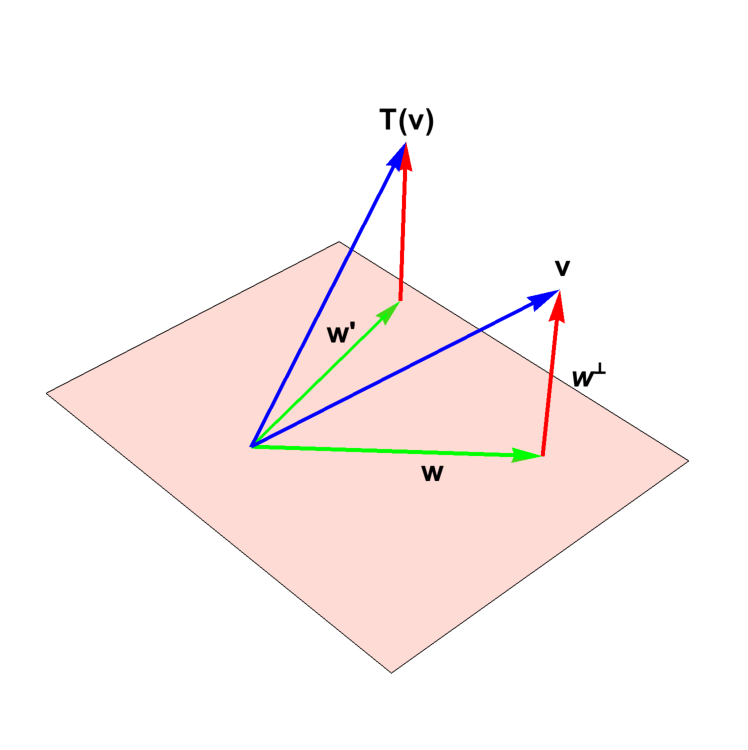
\includegraphics[width=2in]{GeneralRotation}
%\]
%Since rotation is an isometry that fixes the origin, $T$ is linear. As such we wish to come up with the matrix $A$ such that $T=T_A$. Below I outline two different methods. 
%\\
%(a) {\em Method 1}. Create a basis $B'$ of the form $\ds B'=\{ \boldw_1,\boldw_2,\boldn \}$, where $\boldw_1, \boldw_2$ are two orthonormal vectors in $W$. Compute $[T]_{B'}$ then convert everything to the standard basis $B$ using the change of basis formula for transformations. The basis $B'$ being orthonormal simplifies computations. 
%\\  
%(b) {\em Method 2}. (Requires the cross product) Given $\boldv=(x,y,z)$, describe $T(\boldv)$ in terms of the the three mutually orthogonal vectors  $\boldn$, $\boldw=\proj{\boldv}{W}$, and $\ds\boldw'=\boldn\times\proj{\boldv}{W}$. After some work you can derive the formula 
%\[
%T(\boldv)=\cos(\theta)\boldv+\sin(\theta)(\boldn\times\boldv)+((1-\cos \theta)\boldv\cdot\boldn)\boldn.
%\]
%Writing $\boldn=(a,b,c)$ and evaluating this formula for $T$ at $\boldv=(1,0,0), (0,1,0)$ and $(0,0,1)$ will give us the three columns of our matrix, expressed in terms of $a, b, c$ and $\theta$.  
%\\
%\begin{solution}
%%\ \\
%\noindent
%I'll let you think about this one some more. 
%\end{solution}
\ee
